
\section{Gewei Cao's Computational Experience}
\subsection{Lebenslauf}
\begin{table}[H]
\centering 
\caption{\textbf{Experience of Working with Computer}}
\begin{tabular}{ccc}
\toprule
 Time &  Stage & Tools \\
\midrule
before 2017 & Primary and Middle School  & Microsoft Office \\\hline
\multirow{2}{*}{2017 to 2021} & Dongbei University of  & Microsoft Excel,\\    &  Finance and Economics &   Eviews and SPSS\\ \hline
\multirow{2}{*}{2021 to now} & \multirow{2}{*}{Uni Bonn}  & R, MATLAB, \\ 
 & & Stata and Pyhton\\
\bottomrule
\end{tabular}
\end{table}

\subsection{Experience with R}
\begin{flushleft}
I have used R-Studio since my Master study, learned it at course Econometrics and Computational Statistics. I use R-Studio for data visualization, machine learning and econometrics analysis. For my works you can check at my blog 
\underline{https://geweicao.wixsite.com/karl-s-study-blog} , and my GitHub 
\underline{https://github.com/yudingshechu} , 
in addition, my git notes is at \underline{https://github.com/yudingshechu/Effective-Programming-Practice-for-Economists } . 
\end{flushleft}
\begin{center}
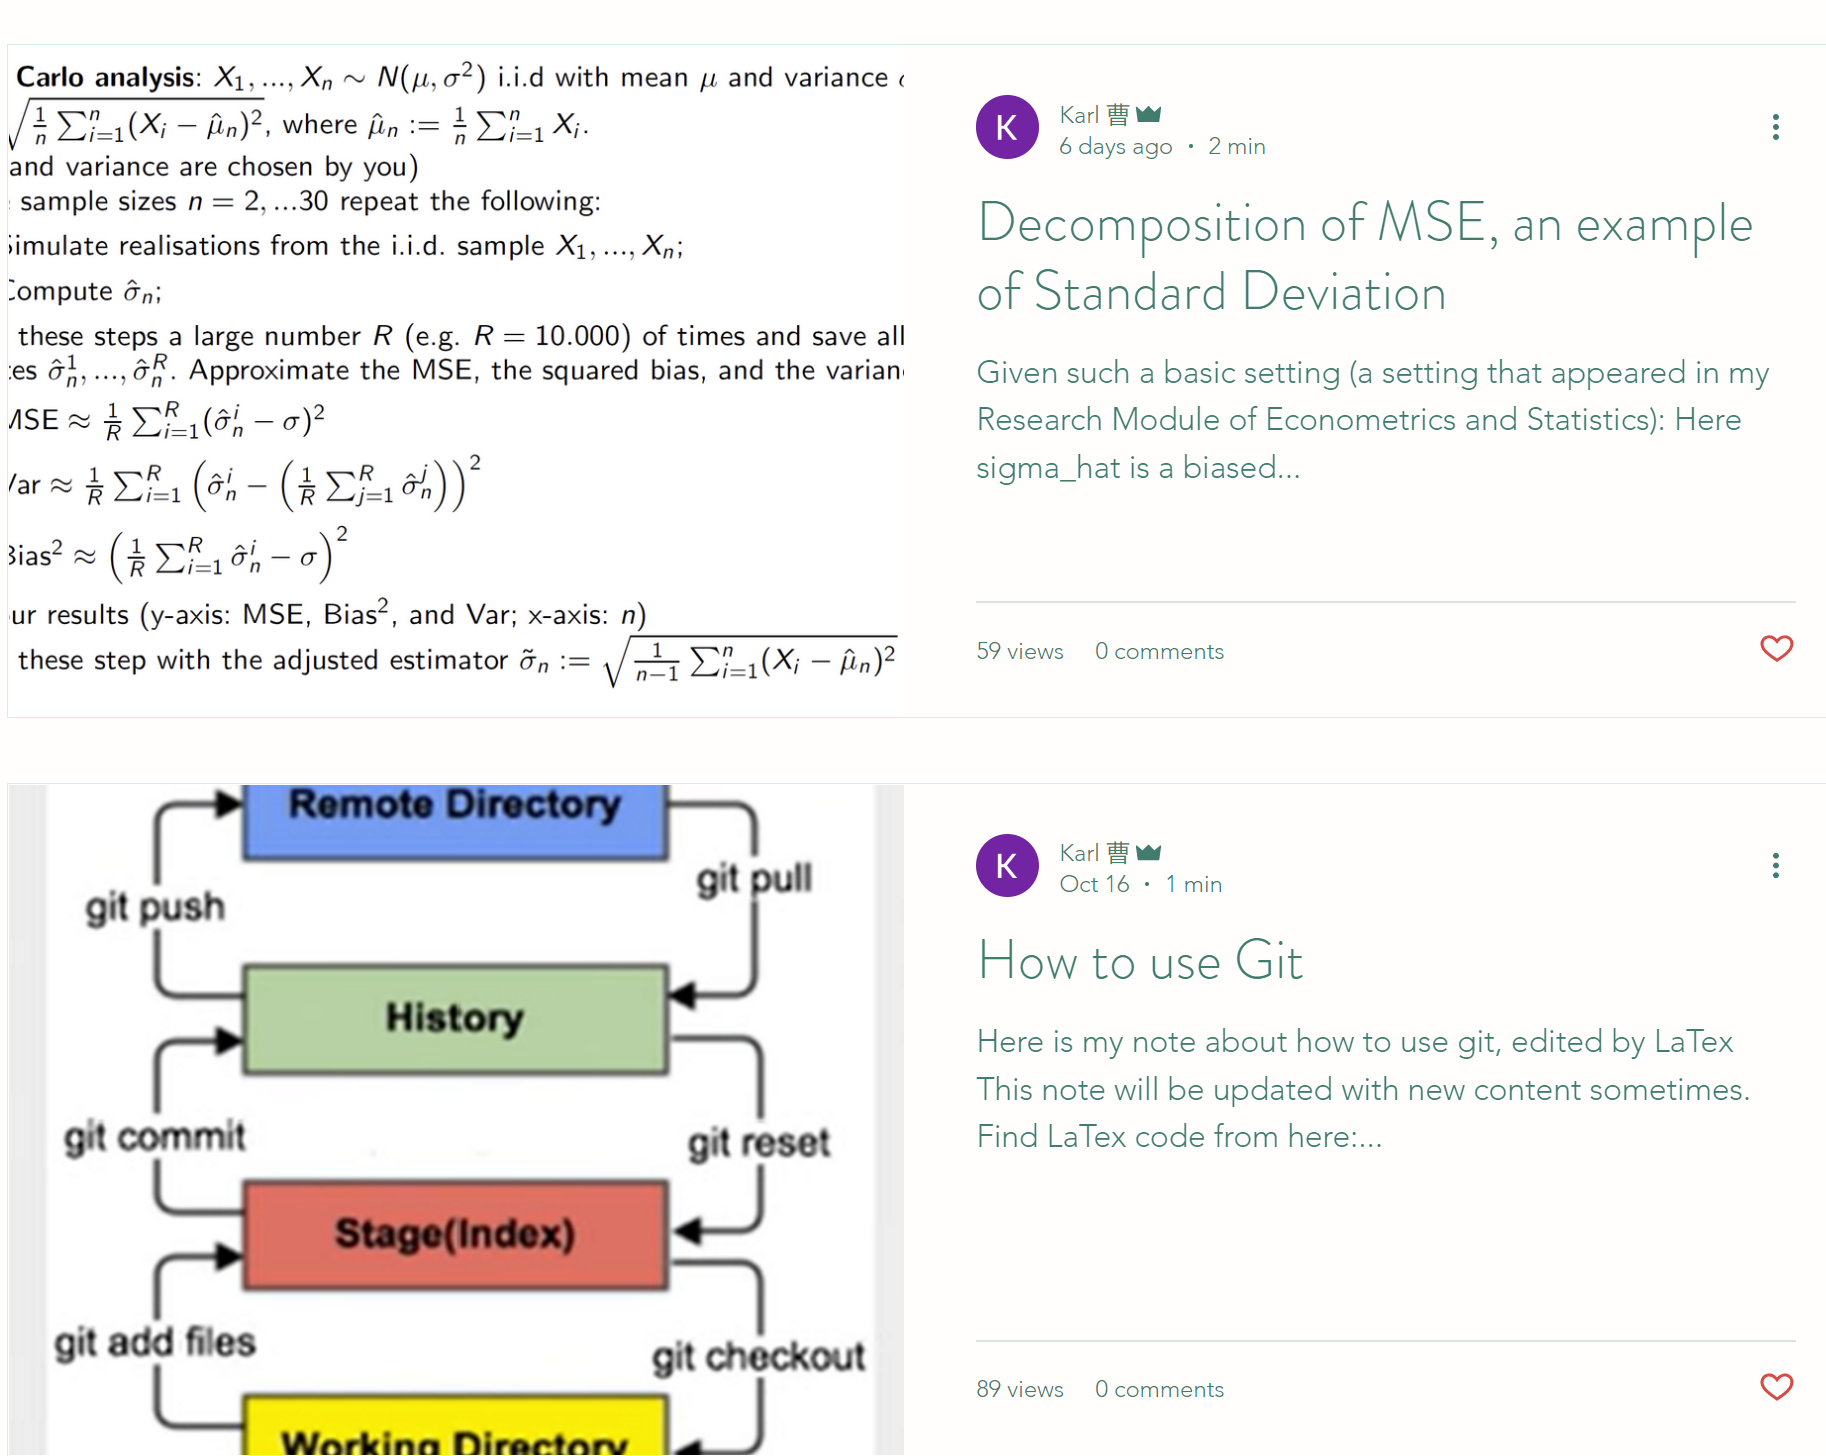
\includegraphics[scale=0.25]{screenshot_ofGewei_blog}
\end{center} 

My final project of Computational Statistics is about Lasso regression in IV regression.
The formula of Lasso is :

\begin{equation*}
\sum_{i = 1}^{n}  ( y_i - \beta_0 \sum_{j = 1}^{p} \beta_j x_ij )^2 + \lambda\sum_{j = 1}^{p} | \beta_j|
\end{equation*}

In addition, I usually use simulated data in R, because I want to control the data generating process, test and compare different algorithms. 

\subsection{Experience with Matlab, Stata}
I used Matlab at basic module of Macroeconomics, and I know how to define functions, write loops in Matlab.\newline

\noindent
I also used Stata at course Empirical Banking and Finance, but I do not know how to manipulate data and write loops with Stata. I get the data from our professor. 

\subsection{Other Experience}
I have used Microsoft Office Word, Powerpoint and Excel since primary school, and during my undergraduate study, I build financial modules with Excel. I used a lot of structured financial data from my Bachelor university's data base and public data base.  \newline

\noindent
I am learning Python at this semester, and I hope I can master it after this course and my self study. About sharing and group working, I prefer to show and share my code, works and ideas with my colleagues. 





